% Copyright 2004 by Till Tantau <tantau@users.sourceforge.net>.
%
% In principle, this file can be redistributed and/or modified under
% the terms of the GNU Public License, version 2.
%
% However, this file is supposed to be a template to be modified
% for your own needs. For this reason, if you use this file as a
% template and not specifically distribute it as part of a another
% package/program, I grant the extra permission to freely copy and
% modify this file as you see fit and even to delete this copyright
% notice. 
\documentclass{beamer}
\usepackage[croatian]{babel}
\usepackage[utf8]{inputenc}
\usepackage{subfig}

% There are many different themes available for Beamer. A comprehensive
% list with examples is given here:
% http://deic.uab.es/~iblanes/beamer_gallery/index_by_theme.html
% You can uncomment the themes below if you would like to use a different
% one:
%\usetheme{AnnArbor}
%\usetheme{Antibes}
%\usetheme{Bergen}
%\usetheme{Berkeley}
%\usetheme{Berlin}
%\usetheme{Boadilla}
%\usetheme{boxes}
%\usetheme{CambridgeUS}
%\usetheme{Copenhagen}
%\usetheme{Darmstadt}
%\usetheme{default}
%\usetheme{Frankfurt}
%\usetheme{Goettingen}
%\usetheme{Hannover}
%\usetheme{Ilmenau}
%\usetheme{JuanLesPins}
%\usetheme{Luebeck}
\usetheme{Madrid}
%\usetheme{Malmoe}
%\usetheme{Marburg}
%\usetheme{Montpellier}
%\usetheme{PaloAlto}
%\usetheme{Pittsburgh}
%\usetheme{Rochester}
%\usetheme{Singapore}
%\usetheme{Szeged}
%\usetheme{Warsaw}

\makeatletter
\newcommand\titlegraphicii[1]{\def\inserttitlegraphicii{#1}}
\titlegraphicii{}
\setbeamertemplate{title page}
{
  \vbox{}
   {\usebeamercolor[fg]{titlegraphic}\inserttitlegraphic\hfill\inserttitlegraphicii\par}
  \begin{centering}
    \begin{beamercolorbox}[sep=8pt,center]{institute}
      \usebeamerfont{institute}\insertinstitute
    \end{beamercolorbox}
    \begin{beamercolorbox}[sep=8pt,center]{title}
      \ifx\insertsubtitle\@empty%
      \else%
        \vskip0.25em%
        {\usebeamerfont{subtitle}\usebeamercolor[fg]{subtitle}\insertsubtitle\par}%
      \fi%     
        \usebeamerfont{title}\inserttitle\par%
    \end{beamercolorbox}%
    \vskip1em\par
        \begin{beamercolorbox}[sep=8pt,center]{author}
      \usebeamerfont{author}\insertauthor
    \end{beamercolorbox}
    \begin{beamercolorbox}[sep=8pt,center]{date}
      \usebeamerfont{date}\insertdate
    \end{beamercolorbox}%\vskip0.5em
  \end{centering}
  %\vfill
}
\makeatother
\author{Filip Gulan}
\title{Očitavanje rukom pisanih slova}
\subtitle{Diplomski seminar}
\institute[FER]{Sveučilište u Zagrebu \\ Fakultet elektrotehnike i računarstva}
\date{Zagreb, svibanj 2017.}
%\titlegraphic{
\includegraphics[height=1cm,width=2cm]{logo}}
%\titlegraphicii{
\includegraphics[height=1cm,width=2cm]{logo}}

%\title{Fakultet elektrotehnike i računarstva}

%\author{Završni rad br. 4581 \\ Očitavanje rukom pisanih slova}
  
%\institute[FER]{Filip Gulan}% (optional, but mostly needed)

%\date{Zagreb, srpanj 2016.}
%\title{Očitavanje rukom pisanih slova}
%\date{}
% A subtitle is optional and this may be deleted
%\subtitle{Završni rad br. 4581}

%\author{Filip Gulan}
% - Give the names in the same order as the appear in the paper.
% - Use the \inst{?} command only if the authors have different
%   affiliation.

%\institute[FER] % (optional, but mostly needed)
% - Use the \inst command only if there are several affiliations.
% - Keep it simple, no one is interested in your street address.

% - Either use conference name or its abbreviation.
% - Not really informative to the audience, more for people (including
%   yourself) who are reading the slides online
% This is only inserted into the PDF information catalog. Can be left
% out. 

% If you have a file called "university-logo-filename.xxx", where xxx
% is a graphic format that can be processed by latex or pdflatex,
% resp., then you can add a logo as follows:

 \pgfdeclareimage[height=0.5cm]{university-logo}{logo}
 \logo{\pgfuseimage{university-logo}}

% Delete this, if you do not want the table of contents to pop up at
% the beginning of each subsection:
%\AtBeginSubsection[]
%{
 % \begin{frame}<beamer>{Outline}
  %  \tableofcontents[currentsection,currentsubsection]
  %\end{frame}
%}

% Let's get started
\begin{document}

\begin{frame}
\maketitle
\end{frame}

\begin{frame}{Sadržaj}
  \tableofcontents
\end{frame}

% Section and subsections will appear in the presentation overview
% and table of contents.

\section{Uvod}
\begin{frame}{Uvod}
  \begin{itemize}
      \item {
        Sustav za prepoznavanje rukom pisanih slova.
      }
      \item{
        Uporaba: automatsko ispravljanje obrazaca s odgovorima na ispitu.
      }
      \item{
        Prikupljanje skupa podataka - obrasci.
      }
      \item{
        Obrada pojedinog slova
      }
      \item{
        Klasifikacija: konvolucijska neuronska mreža.
      }
  \end{itemize}
\end{frame}

\section{Pretprocesiranje slike}

\subsection{Binarizacija}

% You can reveal the parts of a slide one at a time
% with the \pause command:
\begin{frame}{Binarizacija}
  \begin{itemize}
  \item {
    Crno-bijela slika.
    \pause % The slide will pause after showing the first item
  }
  \item {
    Dva razreda slikovnih elemenata: prednji plan ili objekt te pozadina.
    \pause % The slide will pause after showing the first item
  }
  \item {   
    Prag binarizacije.
    \pause
  }
  \item {   
    Izbjegavanje ovisnosti o konstantnom pragu - Otsuova metoda.
    \pause
  }
    \item {
    Izračun histograma slike.
  }
  \end{itemize}
\end{frame}

\begin{frame}{Binarizacija}{Prikaz rada algoritma}
  \begin{figure}[htb]
    \centering
    
\includegraphics[width=10cm]{binarization_example.png}
\end{figure}
\end{frame}

\subsection{Segmentacija i skaliranje slova}

\begin{frame}{Segmentacija i skaliranje slova}
  \begin{itemize}
  \item {
    Binarna slika, iznimno lako pronaći pravokutni okvir slova.
    \pause
  }
  \item {
    Pronalazak najbližeg i najdaljeg crnog slikovnog elementa po visini i širini slike.
    \pause
  }
  \item {
    Skaliranje na uniformne dimenzije ($30 \times 30$) - olakšano izlučivanje značajki.
    \pause
  }
  \item{
    Metode skaliranja:
    \begin{itemize}
        \item bilinearna interpolacija,
        \item bikubična interpolacija,
        \item metoda najbližeg susjeda - korištena,
        \item ...
    \end{itemize}
  }
  \end{itemize}
\end{frame}

\begin{frame}{Segmentacija i skaliranje slova}{Prikaz rada algoritma}

\begin{figure}
\centering
\subfloat{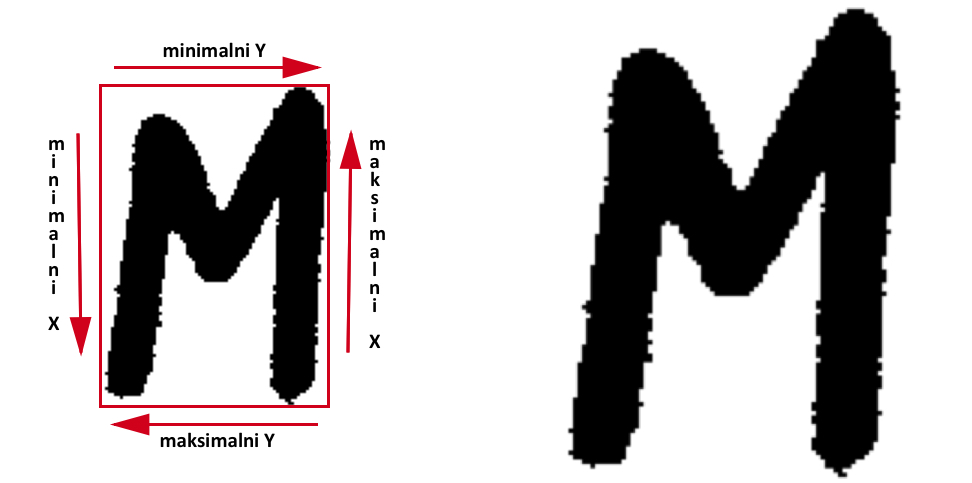
\includegraphics[width=5cm]{crop_example.jpg}}
\subfloat{
\includegraphics[width=4cm]{resize_example.jpg}} 
\end{figure} 

\end{frame}


\section{Konvolucijske neuronske mreže}
\begin{frame}{Konvolucijske neuronske mreže}
\begin{itemize}
  \item {
    Nadogradnja nad višeslojnim unaprijednim neuronskim mrežama.
    \pause
  }
  \item {
    Prilagođene za rad sa slikama.
    \pause
  }
    \item {
    Slojevi:
    \begin{itemize}
        \item Konvolucijski sloj
        \item Sloj sažimanja
        \item Potpuno povezani sloj
    \end{itemize}
    \pause
  }
  \end{itemize}
  \begin{figure}[htb]
    \centering
    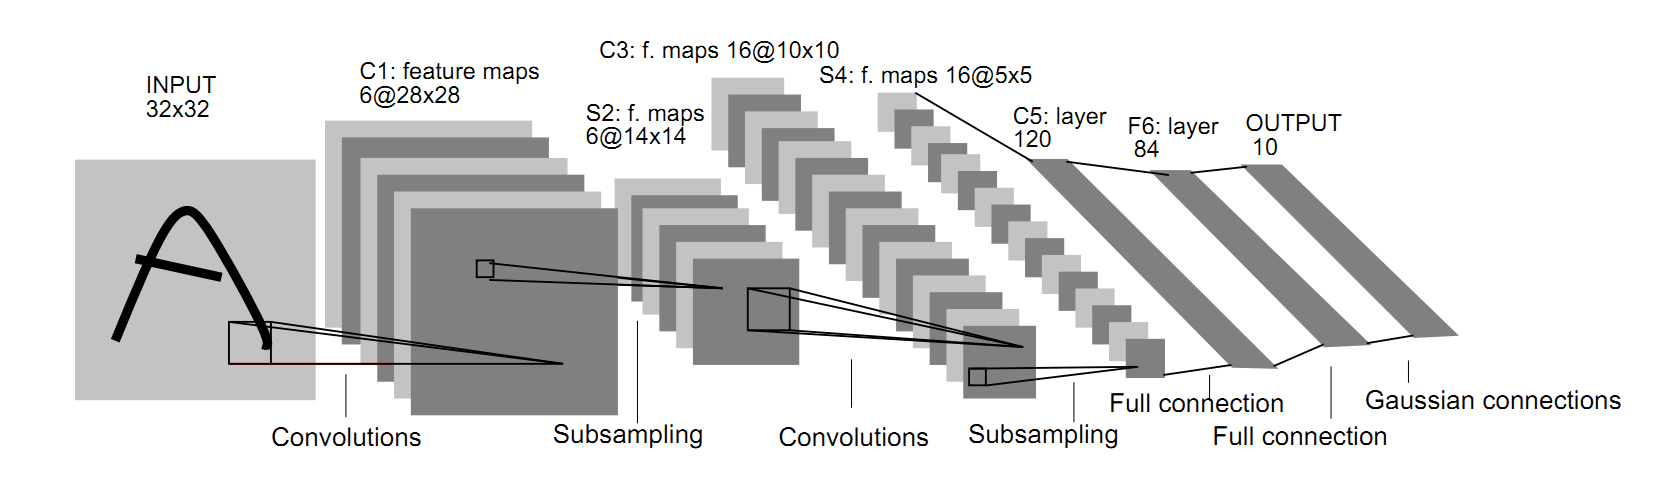
\includegraphics[width=11cm]{lenet-5.png}
    \caption{Konvolucijska neuronska mreža \emph{LeNet-5}, preuzeto iz \emph{Gradient-based learning applied to document recognition, Y. LeCun}}
    \label{fig:lenet5}
    \end{figure}
\end{frame}

\subsection{Konvolucijski sloj}
\begin{frame}{Konvolucijski sloj}
\begin{itemize}
  \item {
    Jezgra funkcionalnosti konvolucijske neuronske mreže.
    \pause
  }
  \item {
    Sastoji se od više filtra.
    \pause
  }
 \item {
    Filtar:
    \begin{itemize}
        \item Prostorna matrica dimenzija $w \times h \times d$
        \item Težine - uče se
    \end{itemize}
    \pause
  }
  \item {
    Konvoluiranje filtra.
    \pause
  }
  \item {
    Izlaz - niz aktivacijskih mapa (odziva filtra).
    \pause
  }
  \item {
  Hiperparametri - broj filtra, veličina filtra, korak pomaka filtra.
  }
\end{itemize}
\end{frame}

\subsection{Sloj sažimanja}
\begin{frame}{Sloj sažimanja}
\begin{itemize}
  \item {
    Cilj: smanjenje prostornih dimenzija ulaza - aktivacijskih mapa.
    \pause
  }
  \item {
    Nakon jednog ili više konvolucijskih slojeva.
    \pause
  }
 \item {
    Vrste:
    \begin{itemize}
        \item Sažimanje srednjom vrijednosti
        \item Sažimanje maksimalnom vrijednosti
        \item Sažimanje L2 normom
        \item Sažimanje težinskim usrednjavanjem
    \end{itemize}
  }
\end{itemize}
  \begin{figure}[htb]
    \centering
    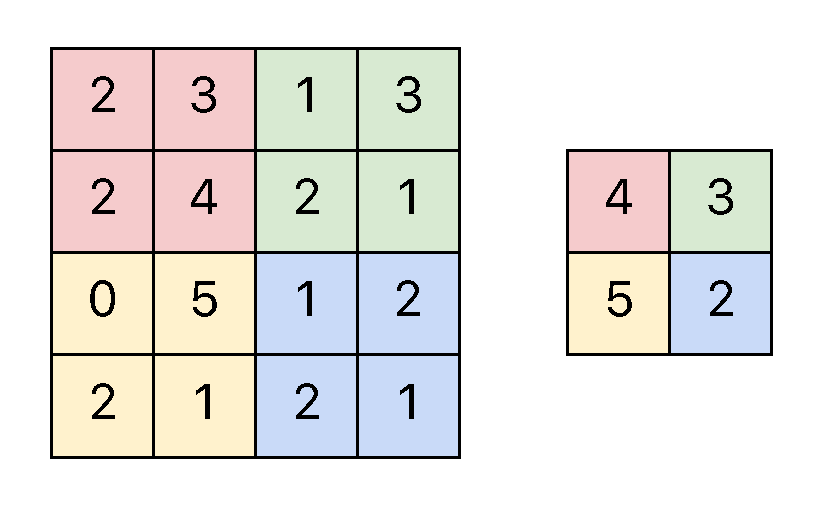
\includegraphics[width=6cm]{pool_example.pdf}
    \end{figure}
\end{frame}

\section{Skup podataka}
\begin{frame}{Skup podataka}
\begin{itemize}
    \item 16 000 slika slova hrvatske i engleske abecede. \pause
    \item 7 750 slika velikih slova, 7 750 slika malih slova, 500 slika znaka "-".
    \pause
    \item Podjela:
        \begin{itemize}
            \item Skup za učenje - 12 000
            \item Skup za provjeru - 4000
            \item Skup za testiranje - 1000
        \end{itemize}
        \pause
    \item Crno-bijele slike - $30 \times 30$.
    \begin{figure}[htb]
    \centering
    
\includegraphics[width=10cm]{dataset_example.pdf}
    \end{figure}
\end{itemize}
\end{frame}

\section{Učenje i rezultati}
\subsection{Arhitektura}
\begin{frame}{Arhitektura}
\begin{itemize}
    \item Konvolucijski sloj: $32$ filtra - $3 \times 3$, korak pomaka - $1$, \emph{ReLU}.
    \item Sloj sažimanja maksimalnom vrijednosti -  $2 \times 2$.
    \item Konvolucijski sloj: $64$ filtra - $3 \times 3$, korak pomaka - $1$, \emph{ReLU}.
    \item Sloj sažimanja maksimalnom vrijednosti -  $2 \times 2$.
    \item Potpuno povezani sloj - $128$ neurona, \emph{ReLU}.
    \item Potpuno povezani sloj - $128$ neurona, \emph{ReLU}.
    \item Izlazni sloj - $32$ neurona, \emph{softmax}.
\end{itemize}
\end{frame}

\subsection{Učenje}
\begin{frame}{Učenje}
\begin{itemize}
    \item \emph{Python, Kreas, TensorFlow} 
    \pause
    \item Algoritam učenja - \emph{ADADELTA}
    \pause
    \item Regularizacija - \emph{dropout}:
        \begin{itemize}
            \item Između potpuno povezanoga sloja i sloja sažimanja - $0.25$
            \item Između dva potpuno povezana sloja - $0.5$
        \end{itemize}
\end{itemize}
\begin{figure}
\centering
\subfloat[][Bez regularizacije]{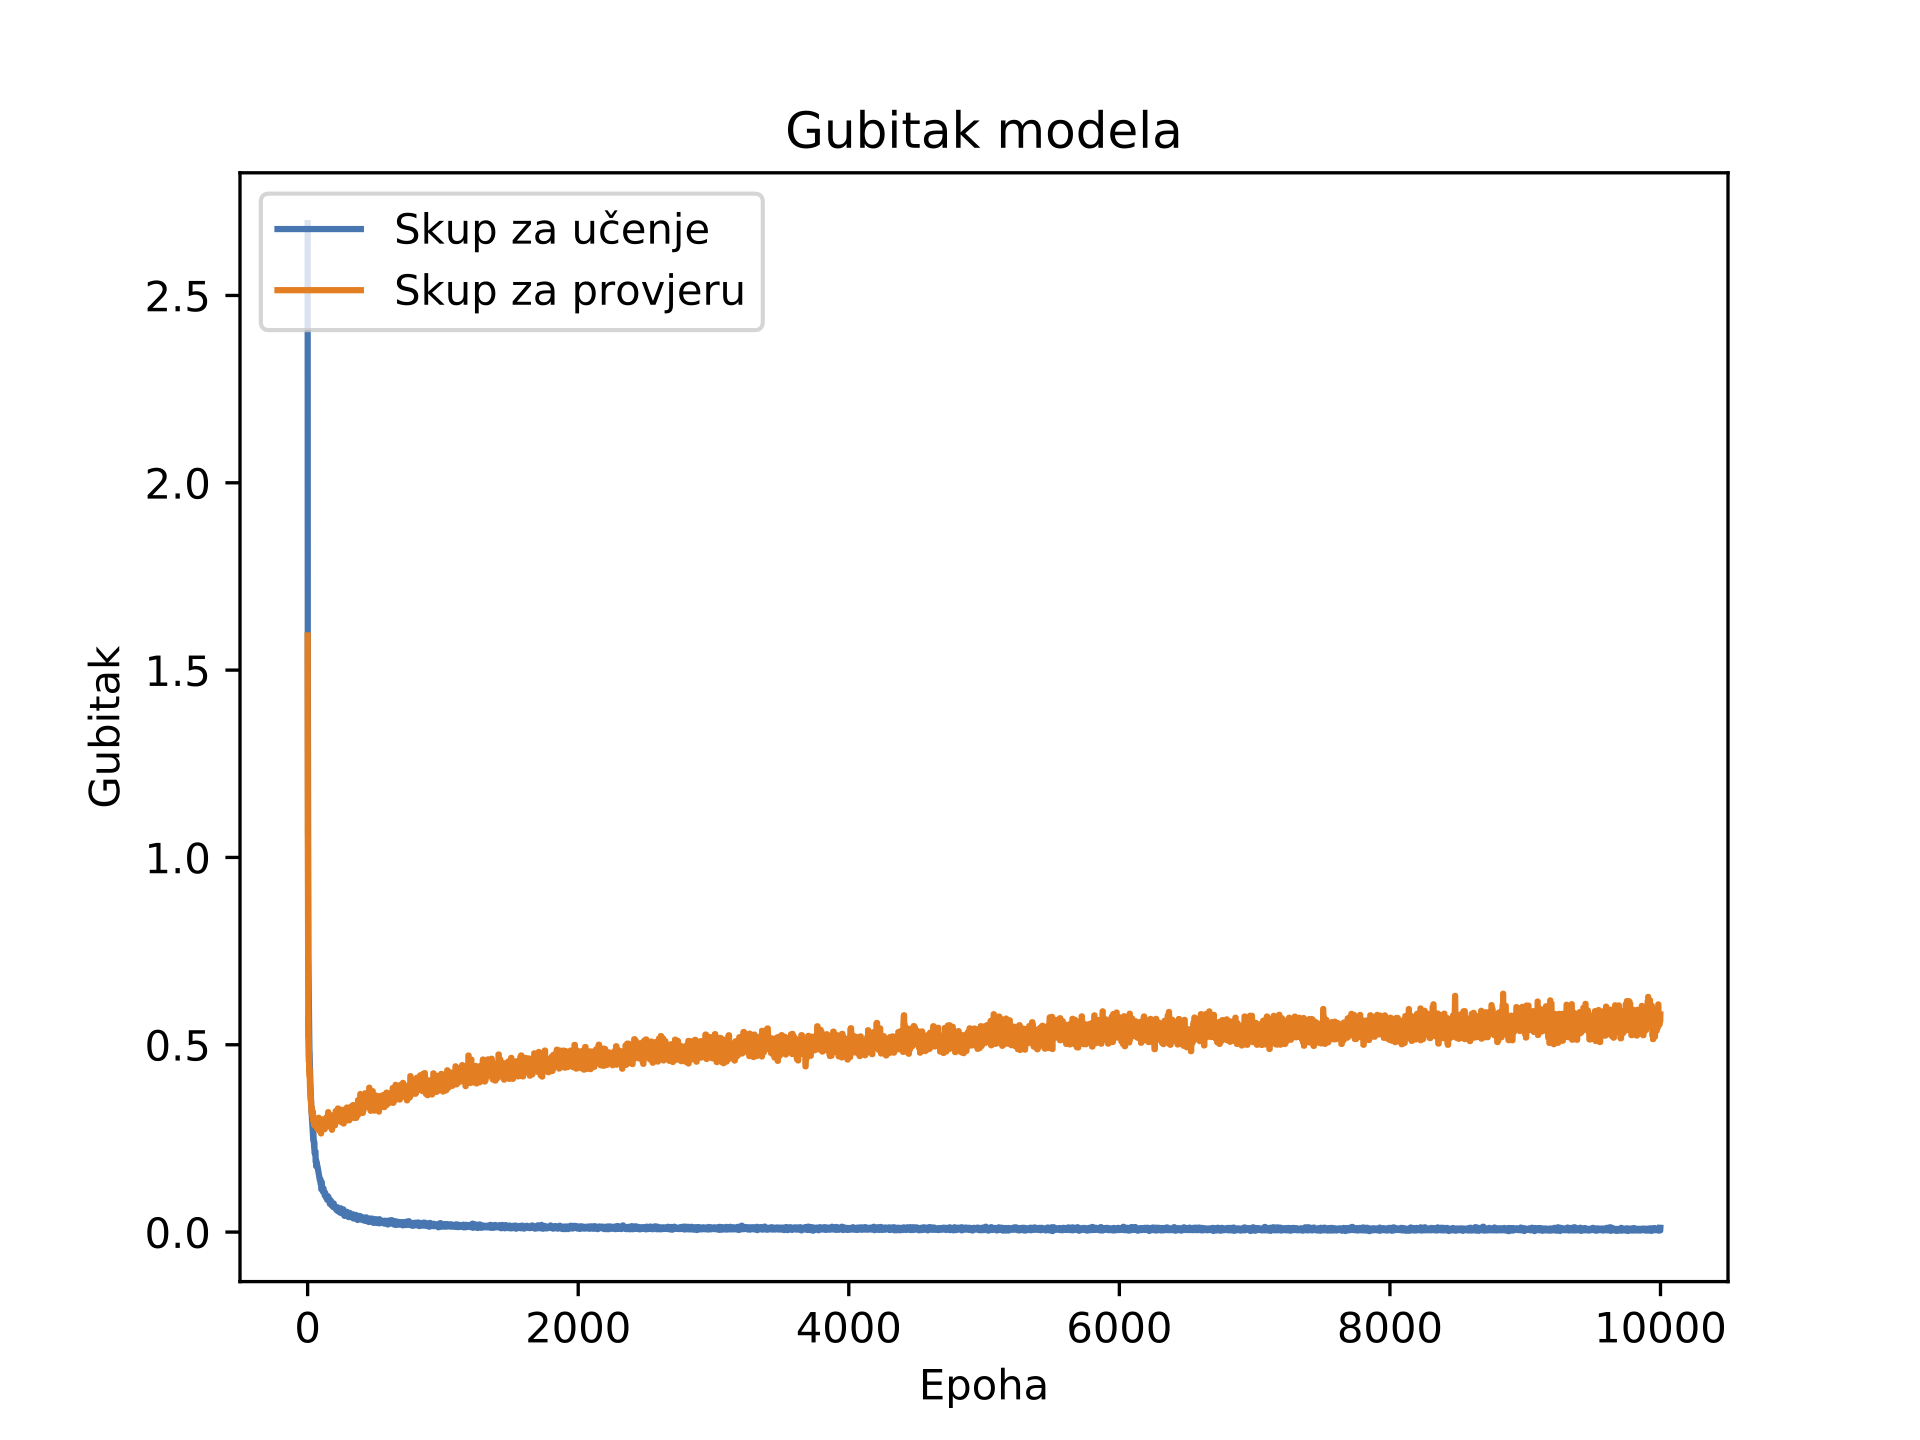
\includegraphics[width=6cm]{overfit.png}}
\subfloat[][Uz regularizaciju]{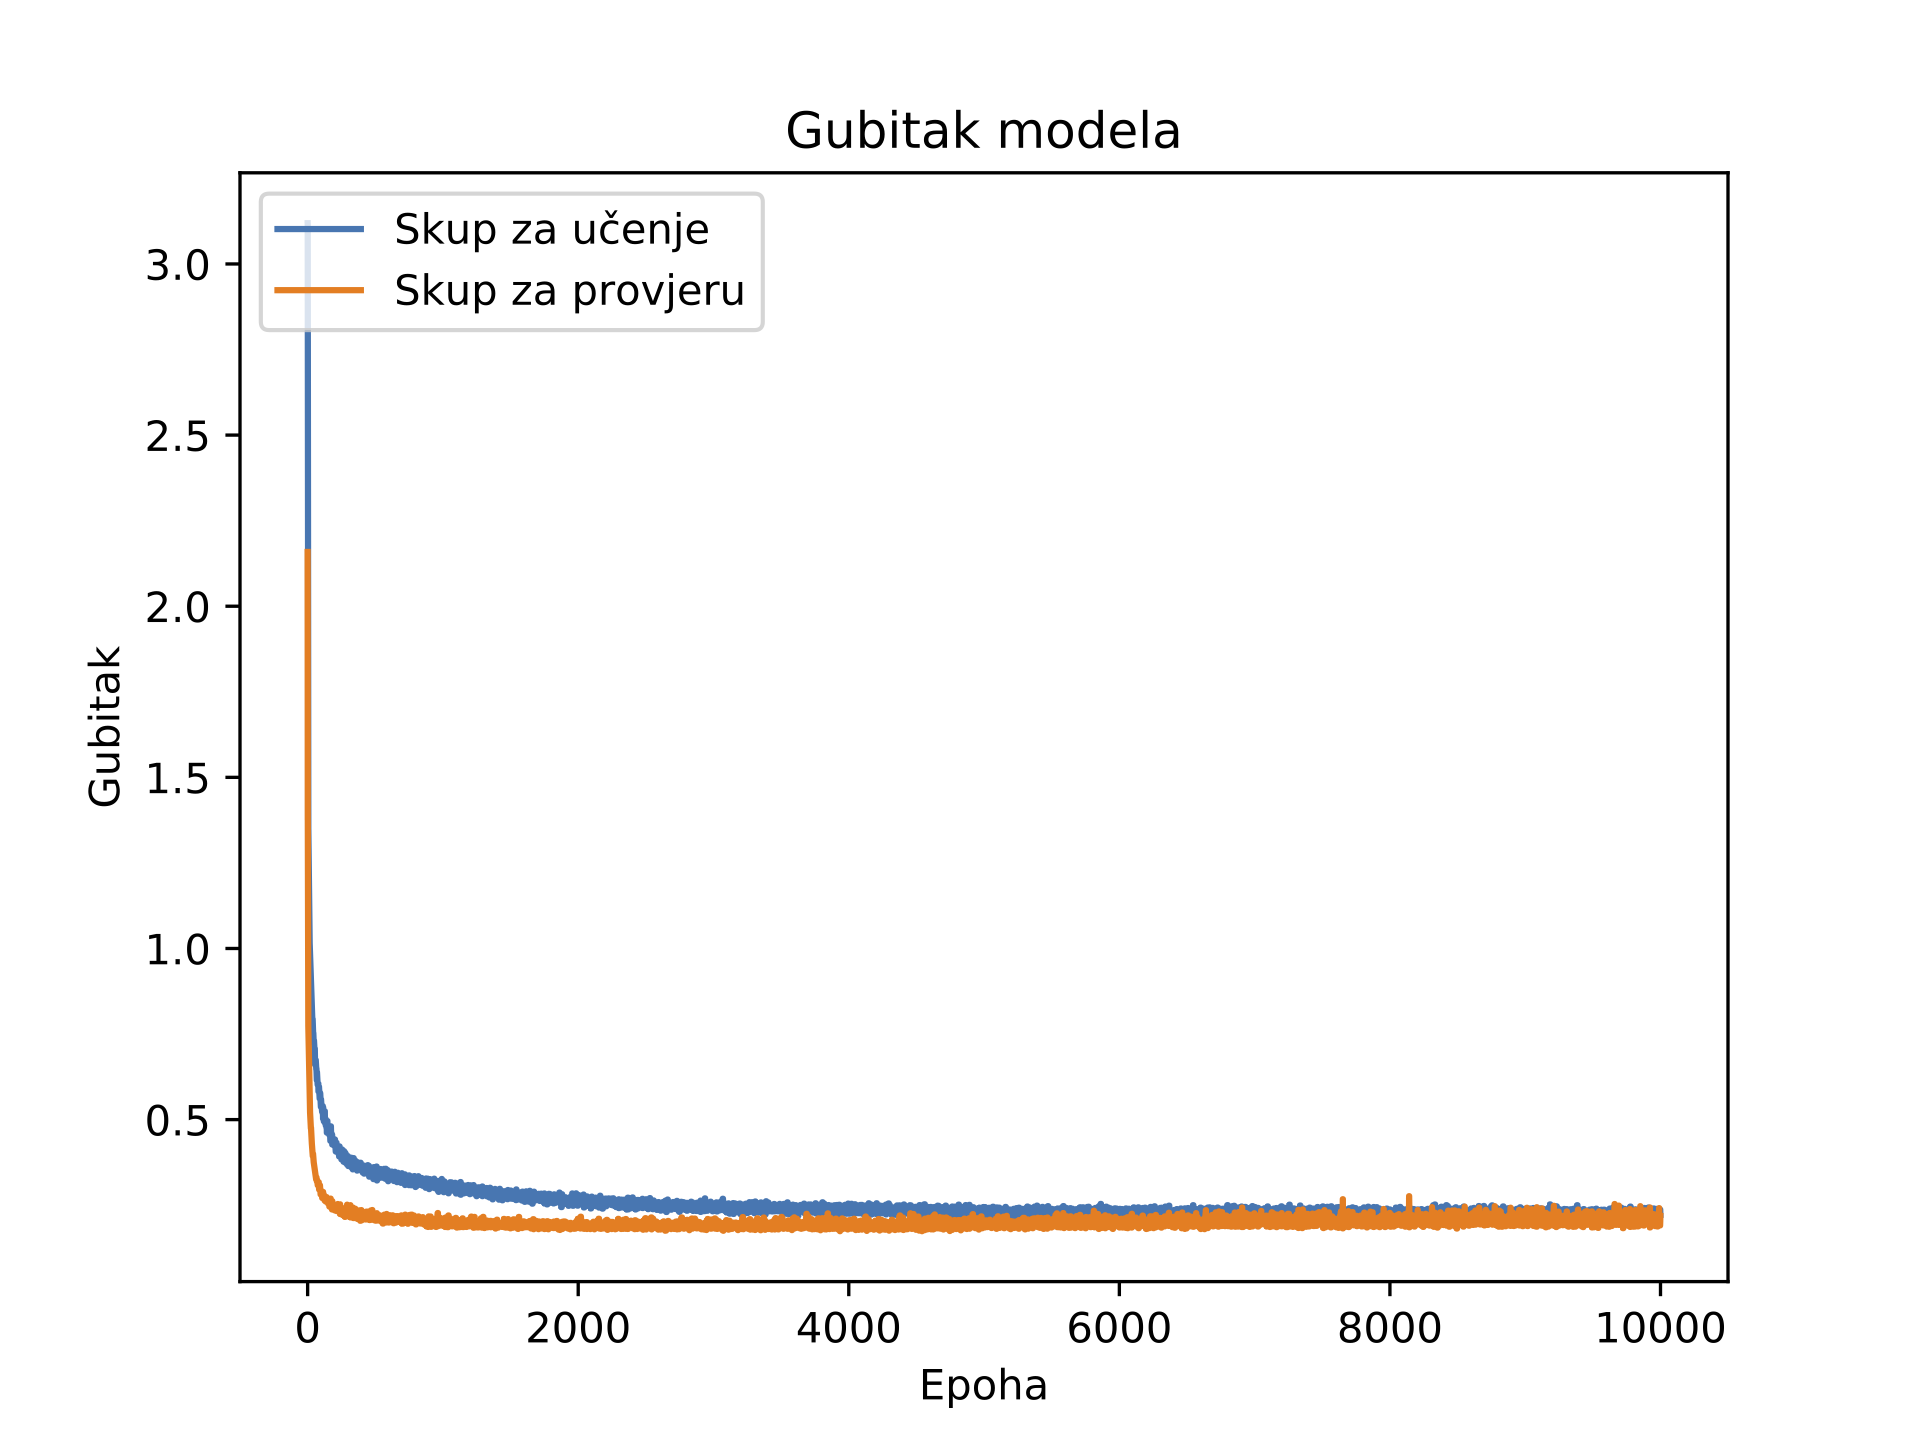
\includegraphics[width=6cm]{model_loss.png}} 
\end{figure} 
\end{frame}

\begin{frame}{Učenje}
\begin{figure}[htb]
    \centering
    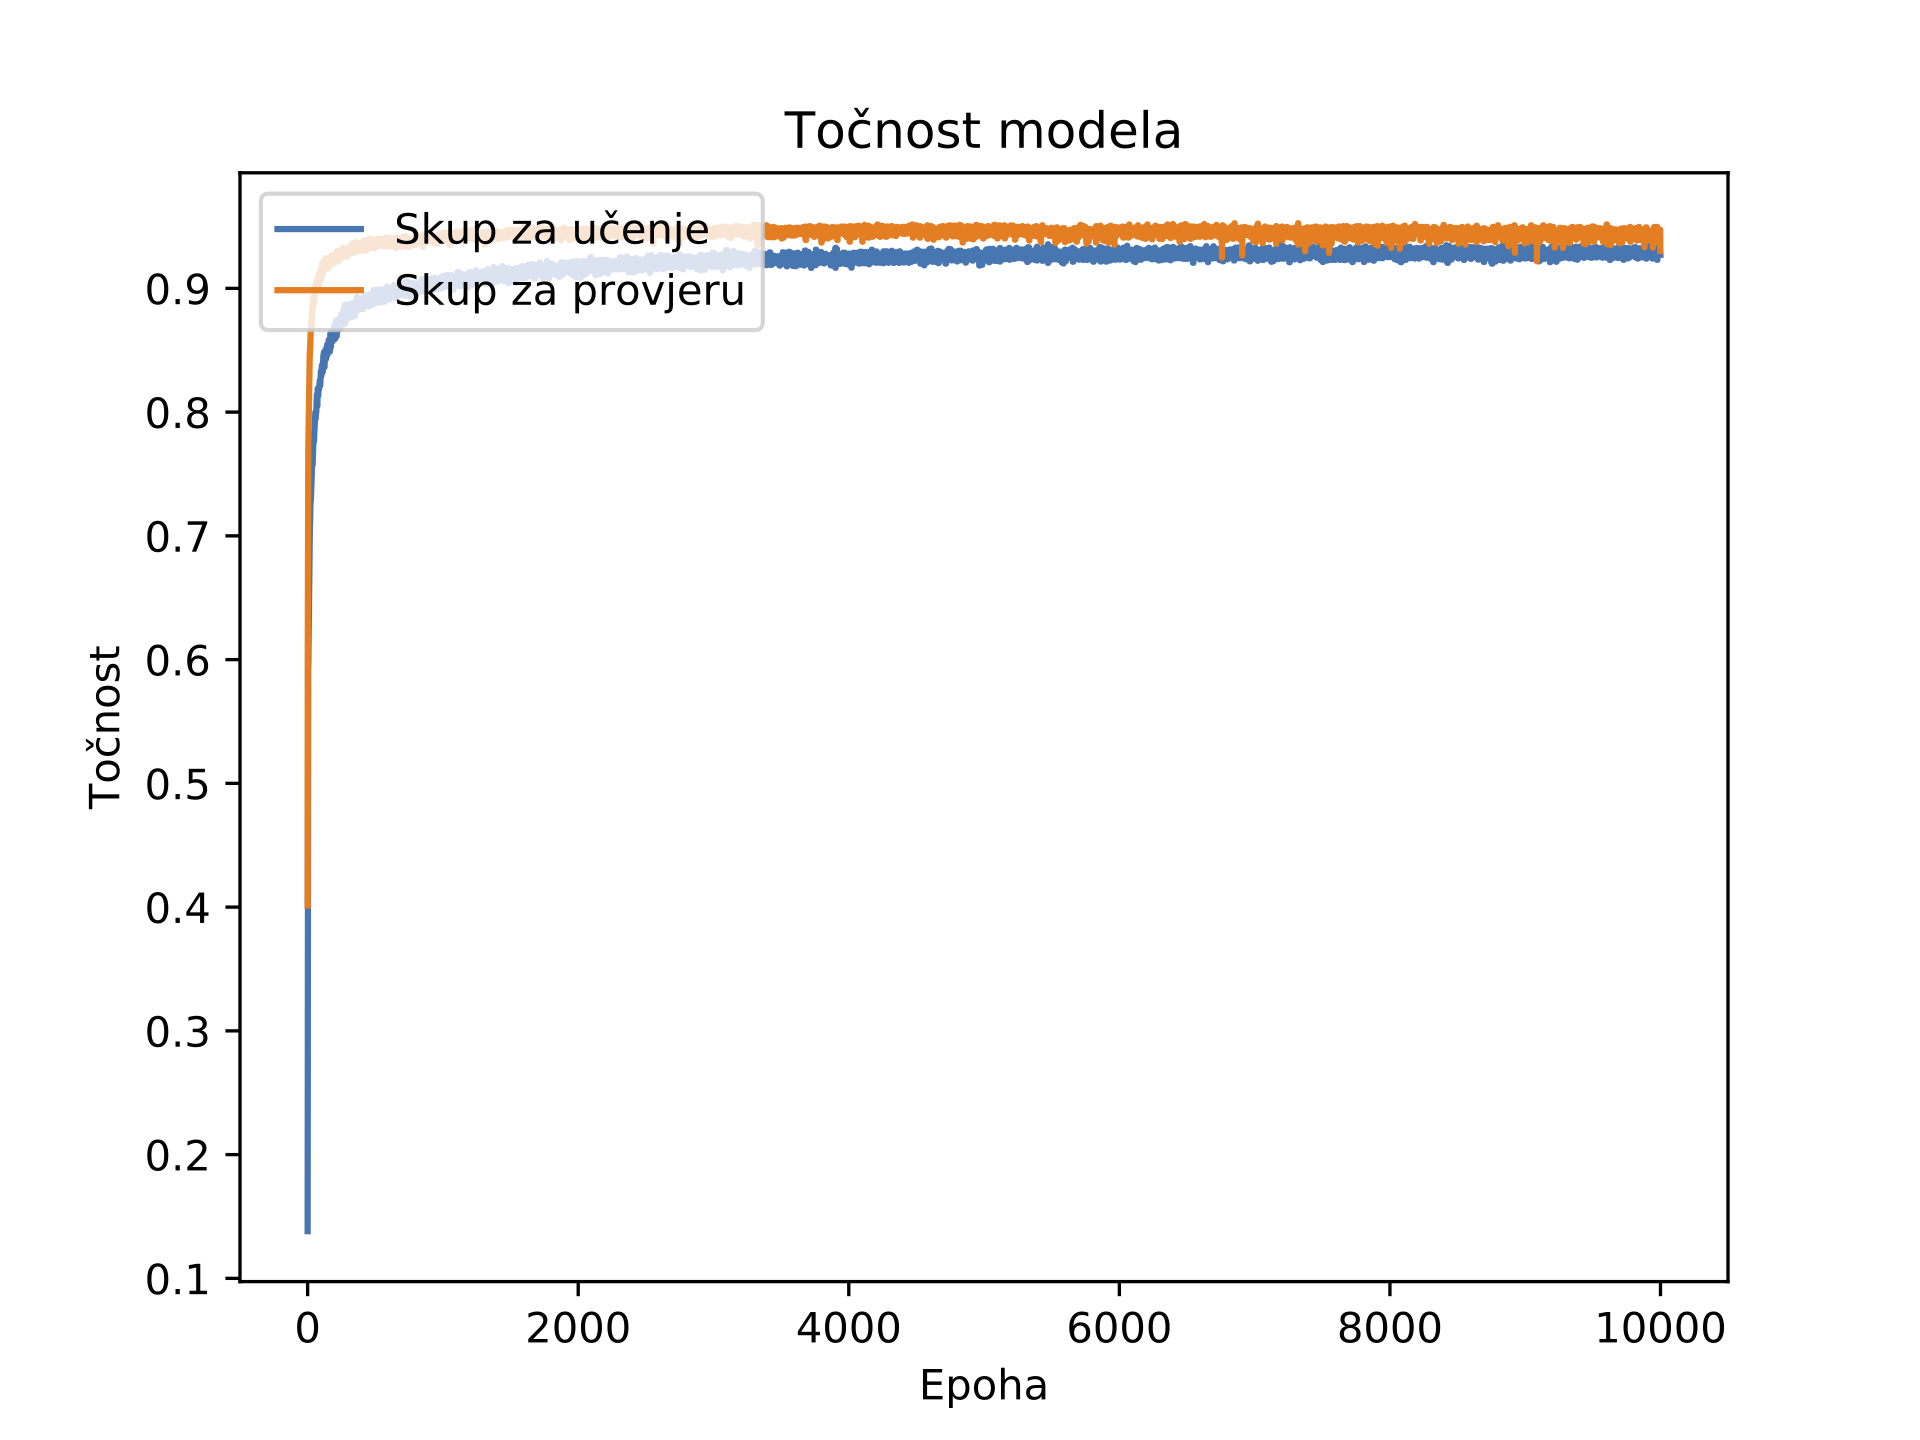
\includegraphics[width=10cm]{model_acc.png}
    \end{figure}
\end{frame}


\begin{frame}{Rezultati}
\begin{table}[]
%\centering
\scalebox{0.95} {
\begin{minipage}{.33\linewidth}
      \centering
        \begin{tabular}{c|c}
Slovo & Točnost \\ \hline
A & 34/35 \\ \hline
B & 31/31 \\ \hline
C & 29/29 \\ \hline
Č & 30/32 \\ \hline
Ć & 28/28 \\ \hline
D & 31/32 \\ \hline
Đ & 27/29 \\ \hline
E & 31/33 \\ \hline
F & 34/35 \\ \hline
G & 30/31 \\ \hline
H & 22/24 \\ \hline
        \end{tabular}
    \end{minipage}
\begin{minipage}{.33\linewidth}
      \centering
        \begin{tabular}{c|c}
Slovo & Točnost \\ \hline
I & 25/31 \\ \hline
J & 21/25 \\ \hline
K & 32/34 \\ \hline
L & 31/39 \\ \hline
M & 32/34 \\ \hline
N & 27/30 \\ \hline
O & 23/24 \\ \hline
P & 26/26 \\ \hline
R & 35/37 \\ \hline
S & 28/32 \\ \hline
Š & 45/45 \\ \hline
        \end{tabular}
    \end{minipage}
\begin{minipage}{.33\linewidth}
      \centering
        \begin{tabular}{c|c}
Slovo & Točnost \\ \hline
T & 47/47 \\ \hline
U & 26/27 \\ \hline
V & 30/32 \\ \hline
Z & 26/27 \\ \hline
Ž & 26/28 \\ \hline
X & 29/29 \\ \hline
Y & 23/24 \\ \hline
W & 23/25 \\ \hline
Q & 23/30 \\ \hline
- & 35/35 \\ \hline
Ukupno & 94\% \\ \hline
        \end{tabular}
    \end{minipage}
}
\caption{Točnost na skupu za testiranje}
\end{table}
\end{frame}

\subsection{Rezultati}
\begin{frame}{Rezultati}
\begin{figure}
\centering
\subfloat{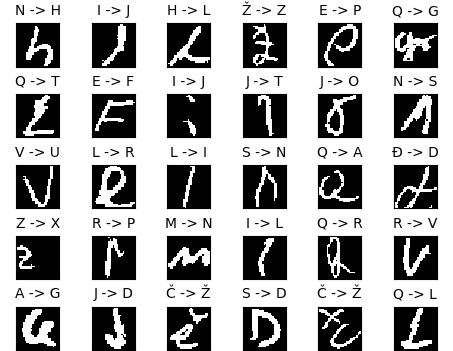
\includegraphics[width=6cm]{wrong.png}}
\subfloat{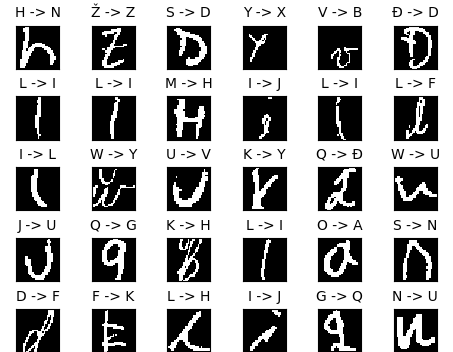
\includegraphics[width=6cm]{wrong2.png}} 
\end{figure} 
\end{frame}

\section*{Zaključak}

\begin{frame}{Zaključak}
  \begin{itemize}
    \item Dobiveni rezultati vrlo zadovoljavajući za dani skup podataka:
     \begin{itemize}
         \item Završni rad - obična neuronska mreža, ručno izlučivanje značajki - $78.44\%$
     \end{itemize}
    \item Potreban veći skup podataka.
    \item Naprednija konvolucijska neuronska mreža.
    \item Poboljšati algoritam učenja.
  \end{itemize}
\end{frame}

\begin{frame}{Kraj}
    \begin{center}
        {\Huge Hvala na pažnji!}
    \end{center}
\end{frame}

\end{document}